% TMUA link-preview diagram: Set B Paper 1, Q7 with the first right-angled
% triangle from its worked solution. Built by og-images/build_tmua.py.
\documentclass[border=12pt]{standalone}
\usepackage{tikz}
\usetikzlibrary{calc}
\definecolor{surface}{RGB}{250,249,246}
\definecolor{accent}{RGB}{118,59,67}
\definecolor{tint}{RGB}{241,232,231}
\pagecolor{surface}
\begin{document}
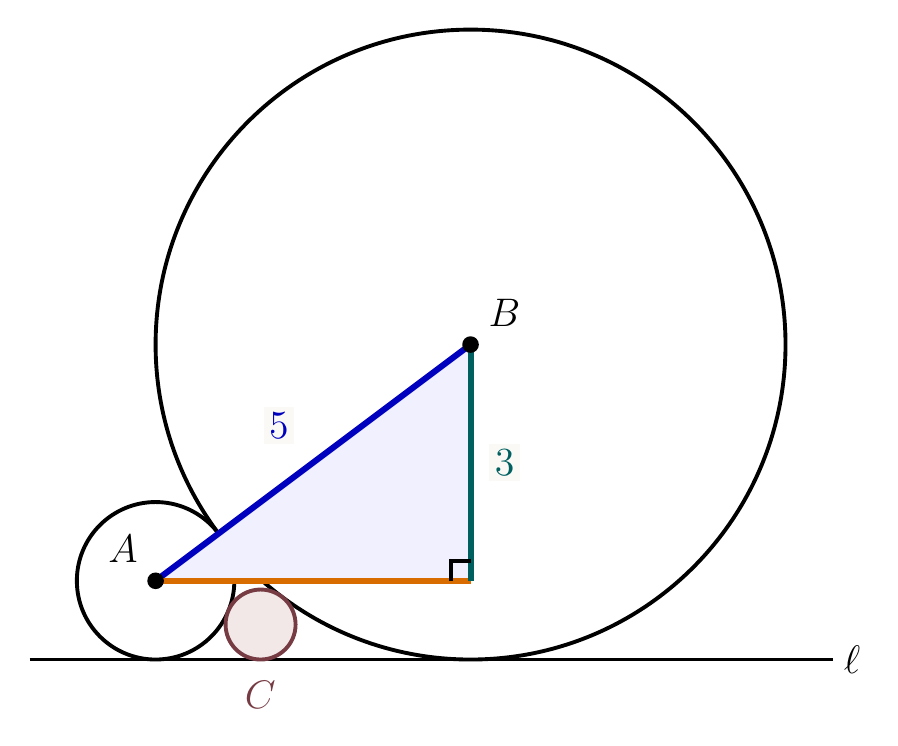
\begin{tikzpicture}[scale=1,every node/.style={font=\Large}]
\coordinate (Acenter) at (0,1);
\coordinate (Bcenter) at (4,4);
\coordinate (ABfoot) at (4,1);
\coordinate (Ccenter) at (4/3,4/9);

\draw[line width=1.4pt,black] (-1.6,0) -- (8.6,0) node[right] {$\ell$};
\draw[line width=1.4pt,black] (Acenter) circle (1);
\draw[line width=1.4pt,black] (Bcenter) circle (4);
\fill[tint] (Ccenter) circle (4/9);
\draw[line width=1.4pt,accent] (Ccenter) circle (4/9);

\fill[blue!6] (Acenter) -- (ABfoot) -- (Bcenter) -- cycle;
\draw[line width=2.2pt,blue!75!black] (Acenter) -- (Bcenter)
    node[midway,above left=2mm,fill=surface,inner sep=2pt] {$5$};
\draw[line width=2.2pt,orange!85!black] (Acenter) -- (ABfoot);
\draw[line width=2.2pt,teal!75!black] (ABfoot) -- (Bcenter)
    node[midway,right=2mm,fill=surface,inner sep=2pt] {$3$};
\draw[line width=1.4pt,black] ($(ABfoot)+(-0.25,0)$) -- ($(ABfoot)+(-0.25,0.25)$) -- ($(ABfoot)+(0,0.25)$);

\fill (Acenter) circle (3pt);
\fill (Bcenter) circle (3pt);
\node[above left=3pt] at (Acenter) {$A$};
\node[above right=3pt] at (Bcenter) {$B$};
\node[accent] at (1.33,-0.45) {$C$};
\end{tikzpicture}
\end{document}
